\providecommand{\GaussCircleArrow}{\ensuremath{\mathord{\vcenter{\hbox{\setlength{\unitlength}{1pt}\begin{picture}(10,11)\linethickness{.55pt}\put(3.3,3.3){\circle{5.2}}\put(5.1,5.1){\line(1,1){3.2}}\put(5.6,8.3){\line(1,0){2.7}}\put(8.3,5.6){\line(0,1){2.7}}\end{picture}}}}}}
\SourceLeaf{482}
auch ist
\[
(\theta,\alpha)=(\theta,-\alpha)
\]
\par\medskip\Needspace{5\baselineskip}\pdfbookmark[1]{Art. 5}{transscendentes-v-art-5}\centerline{[5.]}\nobreak\smallskip
Man setze
\[
\begin{gathered}
\cos\theta=\frac{R(x,y)}{P(x,y)}\,.\,\frac{p}{r},
\\[8pt]\quad{}\qquad i\sin\theta=\frac{S(x,y)}{P(x,y)}\,.\,\frac{q}{r}
\\[8pt]
\cos\tfrac12\theta=\frac{R(x^{\frac12},y^{\frac12})}{\surd 2rP(x,y)},
\\[8pt]\quad{}\qquad i\sin\tfrac12\theta=\frac{S(x^{\frac12},y^{\frac12})}{\surd 2rP(x,y)}
\\[8pt]
y=\cos u+i\sin u
\end{gathered}
\]
dann ist
\[
\begin{gathered}
P(x,y)\,\mathrm{d}\theta=pqQ(x,y)\,\mathrm{d}u
\\[8pt]
\mathrm{d}u=\frac{\mathrm{d}\theta}{\surd(p^4-r^4\cos\theta^2)}
=\frac{\mathrm{d}\theta}{\surd(p^4\sin\theta^2+q^4\cos\theta^2)}
\end{gathered}
\]
\[
\begin{gathered}R(x,y)=x^{\frac14}y^{\frac12}P(x,xy),
\\[8pt]\quad{}\qquad S(x,y)=x^{\frac14}y^{\frac12}Q(x,xy)\end{gathered}
\]
Setzt man
\[
\sin\psi=\frac{rr}{pp}\cos\theta
\]
so wird
\[
\begin{gathered}
\cos\psi=\frac{q}{p}\,.\,\frac{Q(x,y)}{P(x,y)},
\qquad \sin\psi=\frac{r}{p}\,.\,\frac{R(x,y)}{P(x,y)}
\\[8pt]
\mathrm{d}u=-\frac{\mathrm{d}\psi}{\surd(r^4-p^4\sin\psi^2)}
\end{gathered}
\]
\par\medskip\Needspace{5\baselineskip}\pdfbookmark[1]{Art. 6}{transscendentes-v-art-6}\centerline{[6.]}\nobreak\smallskip
\[
\begin{gathered}
P(x,y)\,.\,P(x,z)=P(xx,yz)\,.\,P(xx,\tfrac{y}{z})\\[8pt]\quad{}+R(xx,yz)\,.\,R(xx,\tfrac{y}{z})\\[8pt]
Q(x,y)\,.\,Q(x,z)=P(xx,yz)\,.\,P(xx,\tfrac{y}{z})\\[8pt]\quad{}-R(xx,yz)\,.\,R(xx,\tfrac{y}{z})\\[8pt]
P(x,y)\,.\,Q(x,z)=Q(xx,yz)\,.\,Q(xx,\tfrac{y}{z})\\[8pt]\quad{}+S(xx,yz)\,.\,S(xx,\tfrac{y}{z})\\[8pt]
R(x,y)\,.\,R(x,z)=R(xx,yz)\,.\,P(xx,\tfrac{y}{z})\\[8pt]\quad{}+P(xx,yz)\,.\,R(xx,\tfrac{y}{z})
\end{gathered}
\]
\[
\begin{gathered}P(x,y)^2\,.\,P(x,z)^2+S(x,y)^2\,.\,S(x,z)^2
\\[8pt]\quad{}=Q(x,y)^2\,.\,Q(x,z)^2+R(x,y)^2\,.\,R(x,z)^2\end{gathered}
\]

\SourceLeaf{483}
\par\medskip\Needspace{5\baselineskip}\pdfbookmark[1]{Art. 7}{transscendentes-v-art-7}\centerline{[7.]}\nobreak\smallskip
\[
\begin{gathered}
R(x,1)^7\,.\,P(x^7,y^7)=\text{Product aus}\quad\frac{Fx^{14}}{(Fx^2)^7}\\[8pt]
\quad .\ R(x,1)\,.\,P(x,y)\\[8pt]
\quad .\ \{R(x,\varepsilon)\,.\,P(x,y)-S(x,\varepsilon)\,.\,Q(x,y)\}\\[8pt]
\quad .\ \{R(x,\varepsilon\varepsilon)\,.\,P(x,y)-S(x,\varepsilon\varepsilon)\,.\,Q(x,y)\}\\[8pt]
\quad .\ \{R(x,\varepsilon^3)\,.\,P(x,y)-S(x,\varepsilon^3)\,.\,Q(x,y)\}\\[8pt]
\quad .\ \{R(x,\varepsilon^4)\,.\,P(x,y)-S(x,\varepsilon^4)\,.\,Q(x,y)\}\\[8pt]
\quad .\ \{R(x,\varepsilon^5)\,.\,P(x,y)-S(x,\varepsilon^5)\,.\,Q(x,y)\}\\[8pt]
\quad .\ \{R(x,\varepsilon^6)\,.\,P(x,y)-S(x,\varepsilon^6)\,.\,Q(x,y)\}\\[8pt]
=R(x^7,1)\,.\,P(x,y)^7-\ .\ .\ .\ .\ .\ .\ .\ .\ \\[8pt]\quad{}+7\frac{PQR}{pq}\,.\,P(x,y)\,.\,Q(x,y)^6
\end{gathered}
\]
worin $\varepsilon^7=1$. Zum Beweise dient, was sich leicht nachweisen lässt:
\[
\begin{gathered}
P(x,\varepsilon y)\,.\,P(x,\tfrac{y}{\varepsilon})
=P(xx,yy)\,.\,P(xx,\varepsilon\varepsilon)\\[8pt]\quad{}+R(xx,yy)\,.\,R(xx,\varepsilon\varepsilon)\\[8pt]
=\frac{P(x,y)^2+Q(x,y)^2}{2P(xx,1)}\,.\,P(xx,\varepsilon\varepsilon)
\\[8pt]\quad{}+\frac{P(x,y)^2-Q(x,y)^2}{2R(xx,1)}\,.\,R(xx,\varepsilon\varepsilon)\\[8pt]
=P(x,y)^2\,.\,\frac{R(x,\varepsilon)^2}{R(x,1)^2}
-Q(x,y)^2\,.\,\frac{S(x,\varepsilon)^2}{R(x,1)^2}
\end{gathered}
\]
\par\medskip\Needspace{5\baselineskip}\pdfbookmark[1]{Art. 8}{transscendentes-v-art-8}\centerline{[8.]}\nobreak\smallskip
\[
\begin{aligned}
P(x,1)&=p, & \frac{x\,\mathrm{d}p}{p\,\mathrm{d}x}&=p'\\[8pt]
Q(x,1)&=q, & \frac{x\,\mathrm{d}q}{q\,\mathrm{d}x}&=q'\\[8pt]
R(x,1)&=r, & \frac{x\,\mathrm{d}r}{r\,\mathrm{d}x}&=r'
\end{aligned}
\]
\[
\begin{gathered}
\tfrac12p'=x-2xx+4x^3-4x^4+6x^5-8x^6\\[8pt]\quad{}+8x^7-8x^8+13x^9-12x^{10}\ .\ .\\[8pt]
\tfrac12q'=-x-2xx-4x^3-4x^4-6x^5-8x^6\\[8pt]\quad{}-8x^7-8x^8-13x^9-12x^{10}\ .\ .\\[8pt]
4r'=1+8xx-8x^4+32x^6-40x^8+48x^{10}\\[8pt]\quad{}-32x^{12}+64x^{14}-104x^{16}+104x^{18}\ .\ .
\end{gathered}
\]
Coëfficient von $x^{2^\mu a^\alpha b^{\beta}c^\gamma\ .\ .}$ wenn $a,b,c\ .\ .$ Primzahlen, wird
\[
A\frac{a^{\alpha+1}-1}{a-1}\,.\,\frac{b^{\beta+1}-1}{b-1}\,.\,\frac{c^{\gamma+1}-1}{c-1}\ .\ .
\]
[worin für jene drei Reihen folgeweise]
$A=2^\mu(-1)^{\mu+1},\ A=2^\mu,\ A=8(3-2^\mu)$

\SourceLeaf{484}
\[
\begin{gathered}
4p'-4q'=r^4\\[8pt]
4r'-4p'=q^4\\[8pt]
4r'-4q'=p^4
\end{gathered}
\]
\[
\begin{gathered}
\frac{\mathrm{d}px}{px}-\frac{\mathrm{d}px^2}{px^2}
=\frac{\mathrm{d}x}{x}\,.\,\tfrac12(qx)^2\,.\,(rx^2)^2\\[8pt]
\frac{\mathrm{d}px}{px}-\frac{\mathrm{d}px^3}{px^3}
=\frac{\mathrm{d}x}{x}\,.\,\tfrac12(qx)\,.\,(rx)\,.\,(qx^3)\,.\,(rx^3)\\[8pt]
\frac{\mathrm{d}px}{px}-\frac{\mathrm{d}px^4}{px^4}
=\frac{\mathrm{d}x}{x}\,.\,(qx)\,.\,(px^2)^2\,.\,(rx^4)\\[8pt]
\frac{\mathrm{d}px}{px}-\frac{\mathrm{d}px^5}{px^5}
=\frac{\mathrm{d}x}{4x}\,.\,
\frac{r^4qq(pp-3PP)+R^4QQ(25PP-15pp)}{ppqq-5PPQQ}
\end{gathered}
\]
\par\medskip\Needspace{5\baselineskip}\pdfbookmark[1]{Art. 9}{transscendentes-v-art-9}\centerline{[9.]}\nobreak\smallskip
Bei der $5^{\mathrm{plic.}}$ ist (Aug. 29)
\[
\begin{aligned}
pp-PP&= A\,.\,\surd\frac{p}{P}, &5PP-pp&=B\surd\frac{P}{p}\\[8pt]
qq-QQ&=-A\,.\,\surd\frac{q}{Q}, &5QQ-qq&=B\surd\frac{Q}{q}\\[8pt]
\GaussCircleArrow\quad rr-RR&=A\,.\,\surd\frac{r}{R},
&5RR-rr&=-B\surd\frac{R}{r}
\end{aligned}
\]
\[
\begin{gathered}AB=-2ppPP+2qqQQ+2rrRR=[16pqrPQR]^{\frac23},
\\[8pt]\quad{}\qquad\frac{A}{B}=\frac{PQR}{pqr}\end{gathered}
\]
\[
A=2^{\frac43}\,.\,\frac{(PQR)^{\frac56}}{(pqr)^{\frac16}},
\qquad B=2^{\frac43}\,.\,\frac{(pqr)^{\frac56}}{(PQR)^{\frac16}}
\]
also
\[
pp=(QR+qr)\,.\,\mathord{{}^{6}\!\surd}\frac{ppPP}{16qrQR}\quad\text{etc.}
\]
\[
5=-\frac{qr}{QR}+\frac{pr}{PR}+\frac{pq}{PQ}
\]
Siehe weiter unten [Art. 11.]

Für die Ableitung dient u. a.
\[
\begin{gathered}
P(x^5,x^4)\,.\,P(x^5,-xx)
=P(x^{10},-xx)\,.\,P(x^{10},-x^6)\\[8pt]\quad{}+xP(x^{10},-x^4)\,.\,P(x^{10},-x^8)\\[8pt]
P(x^5,-x^4)\,.\,P(x^5,xx)
=P(x^{10},-xx)\,.\,P(x^{10},-x^6)\\[8pt]\quad{}-xP(x^{10},-x^4)\,.\,
P(x^{10},-x^8)
\end{gathered}
\]

\SourceLeaf{485}
also durch Multiplication
\[
\begin{gathered}
Q(x^{10},1)^2\, .\,P(x^{10},-x^8)\, .\,P(x^{10},-x^4)\\[8pt]
\quad=P(x^{10},-xx)^2\, .\,P(x^{10},-x^6)^2\\[8pt]\quad{}-xxP(x^{10},-x^4)^2\, .\,P(x^{10},-x^8)^2
\end{gathered}
\]
\[
\frac{(Fx^{10})^4}{(Fx^{20})^2}
=\frac{(Fx^4)^3(Fx^{10})^2}{Fx^2\, .\,Fx^{20}}
-xx\frac{Fx^2\, .\,(Fx^{20})^3}{Fx^4\, .\,Fx^{10}}
\]
was mit \GaussCircleArrow{} identisch ist, nemlich
\[
p^{\frac16}q^{\frac16}(\tfrac12r)^{\frac26}
P^{\frac{1}{3}}
Q^{\frac{1}{3}}
(\tfrac12R)^{\frac23}=
\]
Auch beweist man leicht
\[
\begin{gathered}
pp=PP+4\{x^{\frac15}+x^{\frac{16}5}+x^{\frac{36}5}+x^{\frac{81}5}+\, .\,.\}
\\[8pt]\quad{}\{x^{\frac45}+x^{\frac95}+x^{\frac{49}5}+x^{\frac{64}5}+\, .\,.\}\\[8pt]
=PP+4xP(x^5,x^4)\, .\,P(x^5,xx)\\[8pt]
=PP+4x\surd\{\tfrac pP\, .\,\tfrac{(Fx^{10})^5}{Fxx}\}\\[8pt]
=PP+4\surd\frac pP\, .\,\frac{\left(\frac{PQR}{2}\right)^{\frac56}}{\left(\frac{pqr}{2}\right)^{\frac16}}
\end{gathered}
\]
\par\medskip\Needspace{5\baselineskip}\pdfbookmark[1]{Art. 10}{transscendentes-v-art-10}\centerline{[10.]}\nobreak\smallskip
Bei der Trisection ist noch, \(p,P\) etc.\ in voriger Bedeutung genommen
und \(P(x^{\frac13},1)=P^0\) gesetzt
\[
\begin{gathered}
\left(\frac{3PP-P^0P^0}{2}\right)^2=p^4-4\left(\frac{pqr}{2}\right)^{\frac43}\\[8pt]
\left(\frac{3QQ-Q^0Q^0}{2}\right)^2=q^4+4\left(\frac{pqr}{2}\right)^{\frac43}
\end{gathered}
\]
Allgemein wenn \(P(x,1),Q(x,1)\) gegeben sind und \(P(x^n,1),Q(x^n,1)\) gesucht werden,
wo \(n\) ungerade, sind dem \(P(x^n,1)\) coordinirt
\(\pm\surd\frac1n\, .\,P(x^{\frac1n},1)\)
oder \(\pm i\surd\frac1n\, .\,P(x^{\frac1n},1)\), je nachdem \(n\) von der Form
\(4k+1\) oder \(4k-1\) ist.
Die Gleichung findet sich leicht aus Entwickelung der Summe der geraden Potenzen
der \(n+1\) Wurzeln.
\par\medskip\Needspace{5\baselineskip}\pdfbookmark[1]{Art. 11}{transscendentes-v-art-11}\centerline{[11.]}\nobreak\smallskip
Setzt man
\[
\begin{gathered}P(x^5,y^5)=\frac{R}{r^5}\, .\,P(x,y)^5
\\[8pt]\quad{}+A\, .\,P(x,y)^3Q(x,y)^2
+\frac{5PQR}{pqr^5}\, .\,P(x,y)Q(x,y)^4\end{gathered}
\]

\SourceLeaf{486}
so ist auch
\[
\begin{gathered}
Q(x^5,y^5)
=\frac{5PQR}{pqr^5}\, .\,P(x,y)^4\, .\,Q(x,y)\\[8pt]
\quad+A\, .\,P(x,y)^2\, .\,Q(x,y)^3
+\frac{R}{r^5}Q(x,y)^5
\end{gathered}
\]
Setzt man hier \(y=1\), so erhält man
\[
\begin{gathered}
Ap^3q^3=Pq-\frac{R}{r^5}\, .\,p^5q
-\frac{5PQR}{r^5}\, .\,q^4\\[8pt]
=Qp-\frac{R}{r^5}\, .\,q^5p
-\frac{5PQR}{r^5}\, .\,p^4
\end{gathered}
\]
woraus die Gleichung weiter zurück [Art.\ 9] folgt
\[
0=pQr-Pqr+pqR-5PQR
\]
daraus
\[
A=\frac{r(p^3P-q^3Q)-(p^4+q^4)R}{ppqqr^5}
\]
\par\medskip\Needspace{5\baselineskip}\pdfbookmark[1]{Art. 12}{transscendentes-v-art-12}\centerline{[12.]}\nobreak\smallskip
\textsc{Theorem.} Wenn der imaginäre Theil von \(t\) und \(\frac1t\) zwischen \(-i\) und
\(+i\) liegt, so ist der reelle Theil von
\[
\left(\frac{Qt}{Pt}\right)^2
\]
positiv.

\noindent\begin{minipage}{.45\linewidth}
Geometrisch zu beweisen
\end{minipage}\hfill
\resizebox{.47\linewidth}{!}{\begin{tikzpicture}[x=1bp,y=-1bp,line cap=round,line join=round]
\path[use as bounding box] (0,0) rectangle (770,270);
\begin{pgfinterruptboundingbox}
\draw[line width=2.5bp] (85,73) -- (727,73);
\draw[line width=2.5bp] (86,221) -- (184,221);
\draw[line width=2.5bp] (251,221) -- (728,221);
\draw[line width=2.5bp] (92,81) -- (91,213);
\draw[line width=2bp] (101,85) .. controls (112,109) and (115,129.0) .. (100,141.0);
\draw[line width=2bp] (100,151.0) .. controls (115,168.0) and (112,187) .. (101,208);
\node[inner sep=0pt,outer sep=0pt,rotate=0] at (72,52) {\scalebox{4}{\ensuremath{i}}};
\node[inner sep=0pt,outer sep=0pt,rotate=0] at (247,38) {\scalebox{4}{\ensuremath{1+i}}};
\node[inner sep=0pt,outer sep=0pt,rotate=0] at (62,140) {\scalebox{4}{\ensuremath{0}}};
\node[inner sep=0pt,outer sep=0pt,rotate=0] at (386,147) {\scalebox{3.65}{\textbf{Raum für }$t$\textbf{ und }$\dfrac1t$}};
\end{pgfinterruptboundingbox}
\end{tikzpicture}
}

Unter dieser Bedingung ist also das arithmetisch geometrische Mittel zwischen
\[
\mu P(\tfrac12t)^2\qquad\qquad\mu Q(\tfrac12t)^2
\]
indem man immer das geometrische Mittel zwischen \(m,n\) so nimmt, dass
\(\frac{\surd mn}{m}\) einen positiven reellen Theil hat,
\[
=\mu
\]
Ein solches Mittel nennen wir das einfachste Mittel.

Ist das einfachste AG.\ Mittel zwischen \(m,n,=\mu\), das zwischen
\(m,\surd(mm-nn),=\frac\mu t\), so ist \(t\) der Canon des Verhältnisses
\(\frac nm\), nemlich

\SourceLeaf{487}
\[
\frac mn=\left(\frac{Qt}{Pt}\right)^2
\]
dann ist das einfachste AG.\ Mittel zwischen \(m\) und \(-n\)
\[
=\frac\mu{1+2it}
\]
und der dazu gehörige Canon
\[
=\frac t{1+2it}=\frac1{\frac1t+2i}
\]

Die Gleichung
\[
\left(\frac{Qt}{Pt}\right)^2=A
\]
hat immer Eine und nur Eine Auflösung in dem Raume
\begin{center}
\resizebox{.48\linewidth}{!}{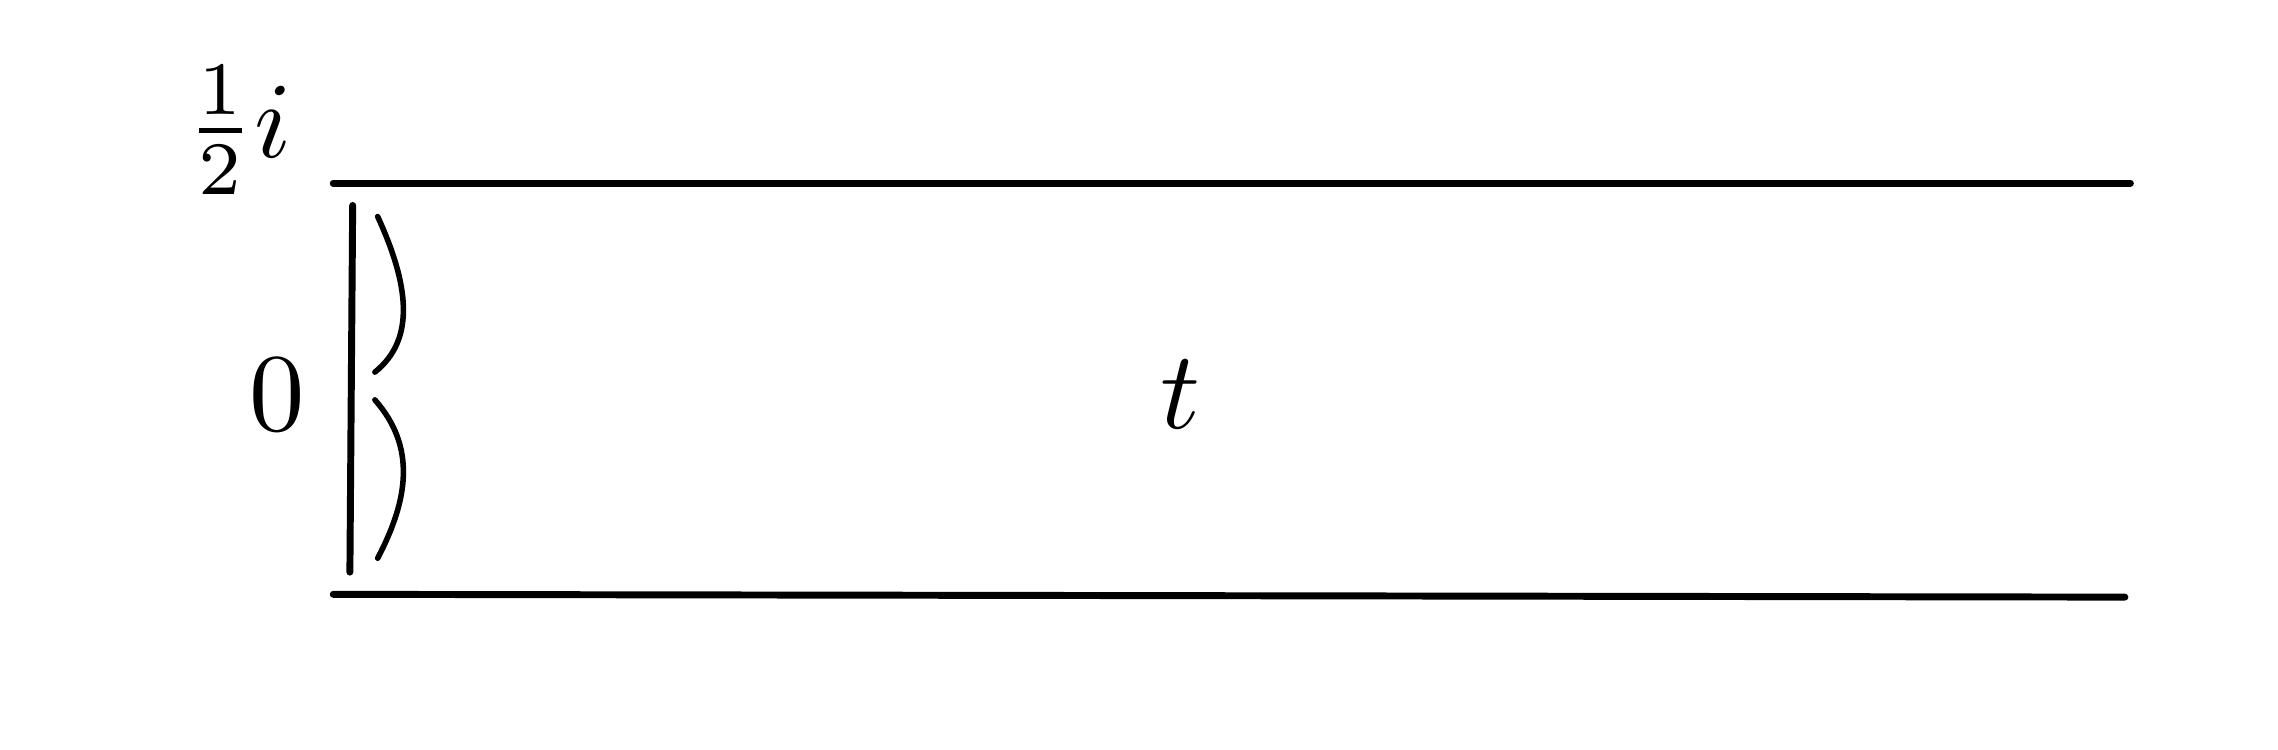
\begin{tikzpicture}[x=1bp,y=-1bp,line cap=round,line join=round]
\path[use as bounding box] (0,0) rectangle (800,250);
\begin{pgfinterruptboundingbox}
\draw[line width=2.5bp] (110,56) -- (757,56);
\draw[line width=2.5bp] (110,204) -- (755,205);
\draw[line width=2.5bp] (117,64) -- (116,196);
\draw[line width=2bp] (126,68) .. controls (137,92) and (140,112.0) .. (125,124.0);
\draw[line width=2bp] (125,134.0) .. controls (140,151.0) and (137,170) .. (126,191);
\node[inner sep=0pt,outer sep=0pt,rotate=0] at (76,37) {\scalebox{3.9}{\ensuremath{\frac12 i}}};
\node[inner sep=0pt,outer sep=0pt,rotate=0] at (90,132) {\scalebox{4}{\ensuremath{0}}};
\node[inner sep=0pt,outer sep=0pt,rotate=0] at (415,132) {\scalebox{4}{\ensuremath{t}}};
\end{pgfinterruptboundingbox}
\end{tikzpicture}
}
\end{center}

Es sei \(\alpha\delta-\beta\gamma=1,\)
\(\alpha\equiv\delta\equiv1\ (\mathrm{mod.}\,4),\)
\(\beta,\gamma\) gerade
\[
t'=i\frac{\alpha t+\beta i}{\gamma t+\delta i}
\]
dann ist
\[
\left(\frac{Qt'}{Pt'}\right)^2=i^\gamma\left(\frac{Qt}{Pt}\right)^2
\]

\par\medskip\Needspace{5\baselineskip}\pdfbookmark[1]{Art. 13}{transscendentes-v-art-13}\centerline{[13.]}\nobreak\smallskip
Fünftheilung
\[
\begin{array}{ll}
a&A\\[8pt]
b&B\\[8pt]
c=\surd(aa-bb)&C=\surd(AA-BB)
\end{array}
\]
\[
2v=-aA+bB+cC
\]
\[
4v=aa-6aA+5AA=-(bb-6bB+5BB)=-(cc-6cC+5CC)
\]
\[
v=-A\surd(AA+v)+B\surd(BB-v)+C\surd(CC-v)
\]

\SourceLeaf{488}

Die Elimination auf eine Gleichung
\[
\surd a+\surd b+\surd c+\surd d=0
\]
angewandt, gibt
\[
0=\Sigma(a^4-4a^3b-2aabb+4aabc-24abcd)
\]

\par\medskip\Needspace{5\baselineskip}\pdfbookmark[1]{Art. 14}{transscendentes-v-art-14}\centerline{[14.]}\nobreak\smallskip
Die $7^{\mathrm{plication}}$ beruht auf
\[
\begin{gathered}
\relax[a\sin(\varphi+A)+b\sin(3\varphi+B)]^2\sin(\varphi+k)\\[8pt]
=\alpha\sin(\varphi+l)
 +\beta\sin(3\varphi+l)
 \\[8pt]\quad{}+\gamma\sin(5\varphi+l)+\delta\sin(7\varphi+l)
\end{gathered}
\]

\par\medskip\Needspace{5\baselineskip}\pdfbookmark[1]{Art. 15}{transscendentes-v-art-15}\centerline{[15.]}\nobreak\smallskip
Bei der Trisection hat man
\[
\surd\frac{q}{p}=n,\qquad \surd\frac{Q}{P}=N
\]
gesetzt,
\[
\frac{N^{4}
 -n^{4}}{1-nnNN}
 =2nN,\qquad
\frac{ppQQ-qqPP}{pP-qQ}=2\surd pPqQ
\]

proportional
\begingroup\small\setlength{\arraycolsep}{1.5pt}\[
\begin{array}{c|l||c|l||c|l}
p^4&3\cos\varphi\sin\varphi^3
&q^4&3\cos(60^0-\varphi)\sin(60^0-\varphi)^3
&r^4&3\cos(120^0-\varphi)\sin(120^0-\varphi)^3\\[8pt]
P^4&\cos\varphi^3\sin\varphi
&Q^4&\cos(60^0-\varphi)^3\sin(60^0-\varphi)
&R^4&\cos(120^0-\varphi)^3\sin(120^0-\varphi)
\end{array}
\]\endgroup

\par\medskip\Needspace{5\baselineskip}\pdfbookmark[1]{Art. 16}{transscendentes-v-art-16}\centerline{[16.]}\nobreak\smallskip
Wenn innerhalb einer begrenzten Figur überall
\[
\frac{\mathrm{dd}V}{\mathrm{d}x^2}
+\frac{\mathrm{dd}V}{\mathrm{d}y^2}=0
\]
an der Grenze hingegen $V$ constant $=A$ ist, so ist nothwendig auch im ganzen Raume $V=A$

Beweis. Es sei $\mathrm{d}M$ ein Element der Fläche und
\[
\begin{gathered}\int\Bigl\{
\Bigl(\frac{\mathrm{d}V}{\mathrm{d}x}\Bigr)^2
+\Bigl(\frac{\mathrm{d}V}{\mathrm{d}y}\Bigr)^2
\\[8pt]\quad{}+\Bigl(\frac{\mathrm{dd}V}{\mathrm{d}x^2}
+\frac{\mathrm{dd}V}{\mathrm{d}y^2}\Bigr)(V-A)
\Bigr\}\mathrm{d}M=\Omega\end{gathered}
\]

\SourceLeaf{489}

Wäre $V$ nicht constant, so wäre offenbar das Integral \emph{positiv}. Allein das Integral ist auch
\[
\int(V-A)\left(\frac{\mathrm{d}V}{\mathrm{d}x}\mathrm{d}y
-\frac{\mathrm{d}V}{\mathrm{d}y}\mathrm{d}x\right)
\]
durch den Umfang der Figur ausgedehnt, also $=0$. Da dies mit dem Vorigen
im Widerspruch steht, so ist die Voraussetzung unzulässig.

Ähnliches findet mit drei Unbestimmten Statt.

Es lassen sich hieraus manche schöne Folgerungen ziehen.

Ein Punkt kann innerhalb eines hohlen Raumes nicht im stabilen Gleichgewicht sein, wenn nicht innerhalb des ganzen Raums gar keine Wirkung Statt
findet, weder im Fall der Abstossung, noch der Anziehung.

\par\medskip\Needspace{5\baselineskip}\pdfbookmark[1]{Art. 17}{transscendentes-v-art-17}\centerline{[17.]}\nobreak\smallskip
Dass in der Peripherie einer Gleichgewichtsfigur keine \emph{negative} Theile sein
können, beweist sich so. Gesetzt $AB$ wäre negativ, so wäre $V-A$ ($A$ Werth
von $V$ in der Peripherie) auswendig neben $AB$ positiv, neben den andern Theilen negativ. Es wird daher einen endlichen Raum geben, wo dies positive gilt;
er sei innerhalb $ABCDE$; dann wäre er aber, da er an der Grenze $0$ ist, in
diesem Raume constant, welches ein Widerspruch.

Dieselbe Schlussart lässt sich auf drei Dimensionen anwenden.

Bei drei Dimensionen findet, für die Fläche $s$, wo $V=\mathrm{Const.}$, noch das
schöne Theorem statt, dass $\int\frac{\mathrm{d}V}{\mathrm{d}\rho}\mathrm{d}s$,
wenn $\rho$ normal gegen $s$, $=4\pi M$, wo $M$
ganze Masse (vermuthlich allemal die in einer solchen Fläche eingeschlossene
Masse, also ungerechnet die draussen liegende).

Vermuthlich ist der Satz für \emph{jede} einhüllende Fläche gültig, ohne dass $V$
constant zu sein braucht.

Es seien zwei einander einschliessende Flächen, in denen $V$ constant ist,
nemlich resp. $V=A$, $V=B$, $\mathrm{d}W$ ein Element des Raumes zwischen beiden,
$p$ die Anziehungskraft in jedem Punkte, dann ist
\[
\int pp\,\mathrm{d}W=(B-A)\, .\,4\pi M
\]
wenn $M$ die Masse im innern Raume, wobei angenommen ist, dass im Raume
$W$ keine anziehende Masse ist.

\par\nopagebreak\begin{center}\rule{93.96bp}{0.35pt}\end{center}

